\documentclass[11pt]{article}
\usepackage[margin=1in]{geometry}
\usepackage{amsmath,amssymb,booktabs,graphicx,setspace,caption,hyperref}
\usepackage[T1]{fontenc}
\usepackage{mathpazo}
\setlength{\parindent}{0pt}
\setlength{\parskip}{0.6em}
\captionsetup{font=small,skip=6pt}
\title{Panel MS-AR(1) for the log gap to the United States\\[0.4em]\large Seasonally adjusted real GDP per worker}
\author{}
\date{}
\begin{document}
\maketitle
\section{Model}
The outcome is the log gap to the US in the same calendar quarter,
\begin{equation}
d_{it}=y_{it}-y_{\mathrm{US},t},
\end{equation}
where $y$ is log seasonally adjusted real GDP per worker (period-average USD) from the 2026-09-17 panel. The United States is the numeraire and is dropped from the panel. A country-quarter is kept only if both that country and the US are observed. There is no common time trend: the US path already removes a shared $gt$.
Joint panel Markov-switching AR(1) with three regimes:
\begin{align}
d_{it} &= a_i + z_{it}, \\
z_{i,t+1} &= \bigl(1-\rho(s_{it})\bigr)\mu(s_{it}) + \rho(s_{it})\, z_{it} + \sigma(s_{it})\,\varepsilon_{it}, \\
s_{i,t+1} &\sim \Pi(\,\cdot\mid s_{it}), \\
a_i &\sim \mathcal{N}(\alpha,\omega^2).
\end{align}
Spec 1 is this model. Spec 2 keeps the permanent gap and adds a decaying entry deviation from that gap,
\begin{align}
d_{it} &= a_i + b_i\,\lambda^{t-T_{i0}} + z_{it}, \\
b_i &\sim \mathcal{N}(0,\omega_b^2) \ \text{independent of } a_i,
\end{align}
with $\lambda=0.98$ fixed (Barro 2\% per year). $T_{i0}$ is country $i$'s first observation. The long-run gap is $a_i$. Random effects are integrated by Gauss--Hermite quadrature (11-point in spec 1; $7\times 7$ in spec 2). Plotted cycles use posterior-mean $a_i$ (and $b_i$ in spec 2). Latent paths $s_{it}$ are country-specific. $\sigma$ and $\rho$ switch. The median $\mu$ is pinned at 0. $|\rho|<0.99$.
Standard errors (in parentheses) are delta-method from a numerical Hessian. $\pi$ is the ergodic distribution of $\Pi$. $E[z]$ is the long-run mean of the cycle.
\clearpage
\section{Log gap to the US: random intercepts, no trend}
2026-09-17 SA panel, log gap to the US. 73 countries (USA dropped), 8364 observations, 1963-Q1--2026-Q2. Fitted countries: 73. Observations: 8364. Log-likelihood: 21706.11. Ergodic mean of the cycle $E[z]=0.2281$ (0.0295).
Random intercepts $a_i\sim N(\alpha,\omega^2)$ with $\alpha=-1.7591$ (0.0343), $\omega=0.6689$ (0.0091). Posterior-mean $a_i$: mean -1.669, min -3.675, max 0.157.
\begin{table}[h]
\centering
\caption{Regime AR(1), transition matrix, and ergodic $\pi$. Columns are regimes.}
\begin{tabular}{lccc}
\toprule
 & (0) & (1) & (2) \\
\midrule
$\mu$ & -0.2900 & 0.0000 & 0.4435 \\
 & (0.1637) & --- & (0.0372) \\ \addlinespace
$\sigma$ & 0.0940 & 0.0227 & 0.0093 \\
 & (0.0040) & (0.0007) & (0.0002) \\ \addlinespace
$\rho$ & 0.9900 & 0.9900 & 0.9900 \\
 & (0.0001) & (0.0000) & (0.0000) \\ \addlinespace
$\Pi_{0\cdot}$ & 0.5808 & 0.4104 & 0.0088 \\
 & (0.0440) & (0.0509) & (0.0201) \\ \addlinespace
$\Pi_{1\cdot}$ & 0.0563 & 0.8770 & 0.0666 \\
 & (0.0090) & (0.0134) & (0.0092) \\ \addlinespace
$\Pi_{2\cdot}$ & 0.0133 & 0.0323 & 0.9544 \\
 & (0.0032) & (0.0060) & (0.0051) \\ \addlinespace
$\pi$ & 0.0679 & 0.3733 & 0.5588 \\
 & (0.0076) & (0.0236) & (0.0267) \\ \addlinespace
\bottomrule
\end{tabular}
\end{table}
\begin{figure}[h]
\centering
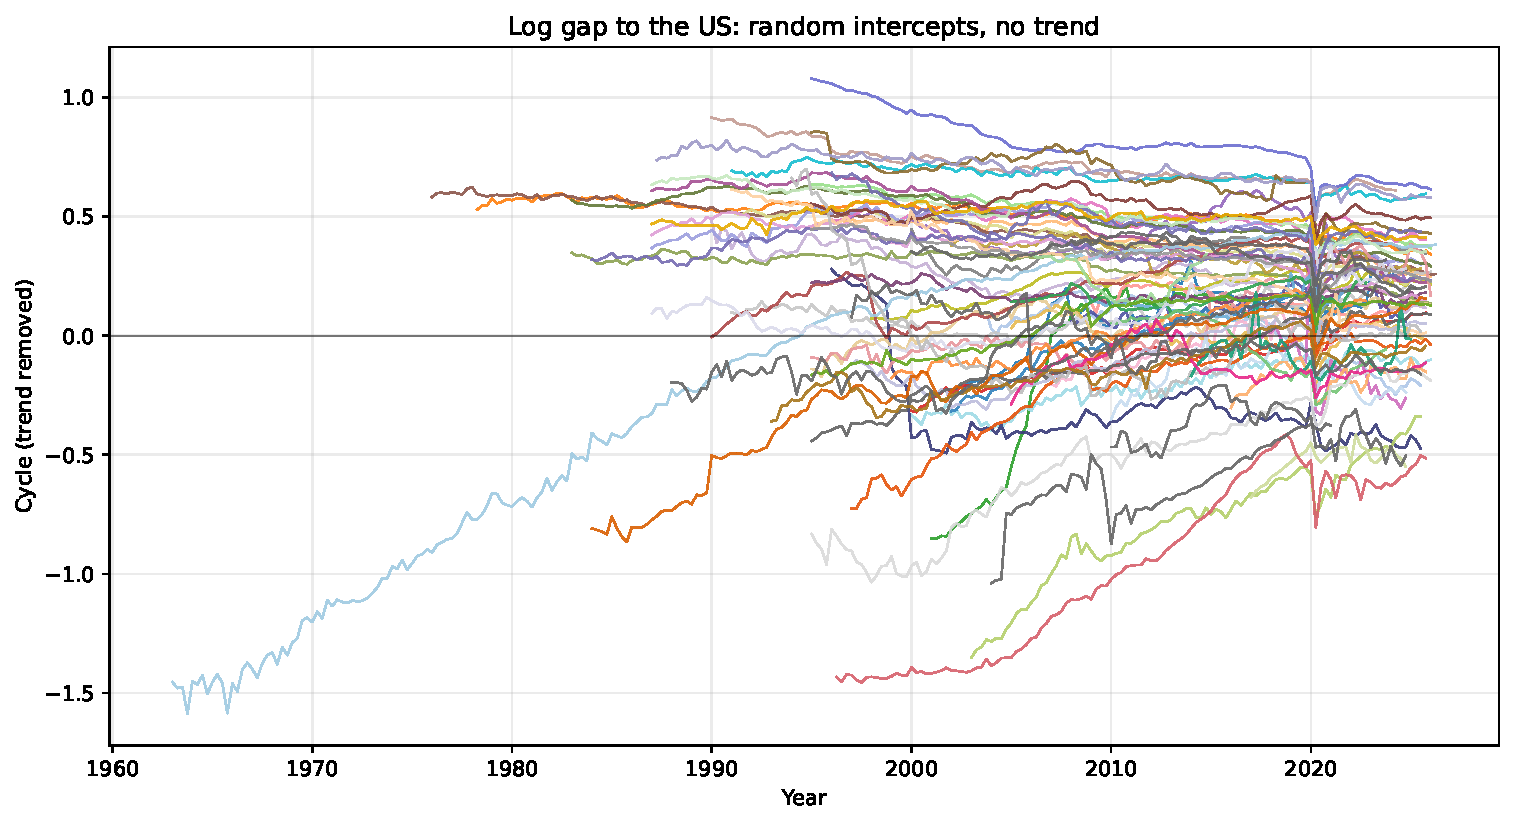
\includegraphics[width=0.75\textwidth]{figs/cycle_gap_re.pdf}
\caption{Country cycles in the US gap after removing the deterministic path.}
\end{figure}
\clearpage
\section{Log gap to the US: RE intercepts plus Barro catch-up}
2026-09-17 SA panel, log gap to the US. 73 countries (USA dropped), 8364 observations, 1963-Q1--2026-Q2. Fitted countries: 73. Observations: 8364. Log-likelihood: 21810.29. Ergodic mean of the cycle $E[z]=0.0284$ (0.0409).
Permanent RE intercepts and catch-up $y_{it}=a_i + b_i\lambda^{t-T_{i0}}+z_{it}$ with $\alpha=-1.4034$ (0.0409), $\omega=0.6483$ (0.0080), $\lambda=0.9800$ (fixed), $\omega_b=0.4701$ (0.0123). Posterior-mean $a_i$: mean -1.495, min -3.834, max 0.132. Posterior-mean $b_i$: mean -0.023, min -1.106, max 1.113.
\begin{table}[h]
\centering
\caption{Regime AR(1), transition matrix, and ergodic $\pi$. Columns are regimes.}
\begin{tabular}{lccc}
\toprule
 & (0) & (1) & (2) \\
\midrule
$\mu$ & -0.9403 & 0.0000 & 0.2559 \\
 & (0.1739) & --- & (0.0408) \\ \addlinespace
$\sigma$ & 0.0910 & 0.0217 & 0.0089 \\
 & (0.0039) & (0.0007) & (0.0002) \\ \addlinespace
$\rho$ & 0.9830 & 0.9900 & 0.9900 \\
 & (0.0052) & (0.0000) & (0.0000) \\ \addlinespace
$\Pi_{0\cdot}$ & 0.5877 & 0.4123 & 0.0000 \\
 & (0.0420) & (0.0420) & (0.0000) \\ \addlinespace
$\Pi_{1\cdot}$ & 0.0544 & 0.8826 & 0.0630 \\
 & (0.0077) & (0.0107) & (0.0076) \\ \addlinespace
$\Pi_{2\cdot}$ & 0.0126 & 0.0338 & 0.9536 \\
 & (0.0030) & (0.0055) & (0.0048) \\ \addlinespace
$\pi$ & 0.0685 & 0.3950 & 0.5365 \\
 & (0.0077) & (0.0238) & (0.0271) \\ \addlinespace
\bottomrule
\end{tabular}
\end{table}
\begin{figure}[h]
\centering
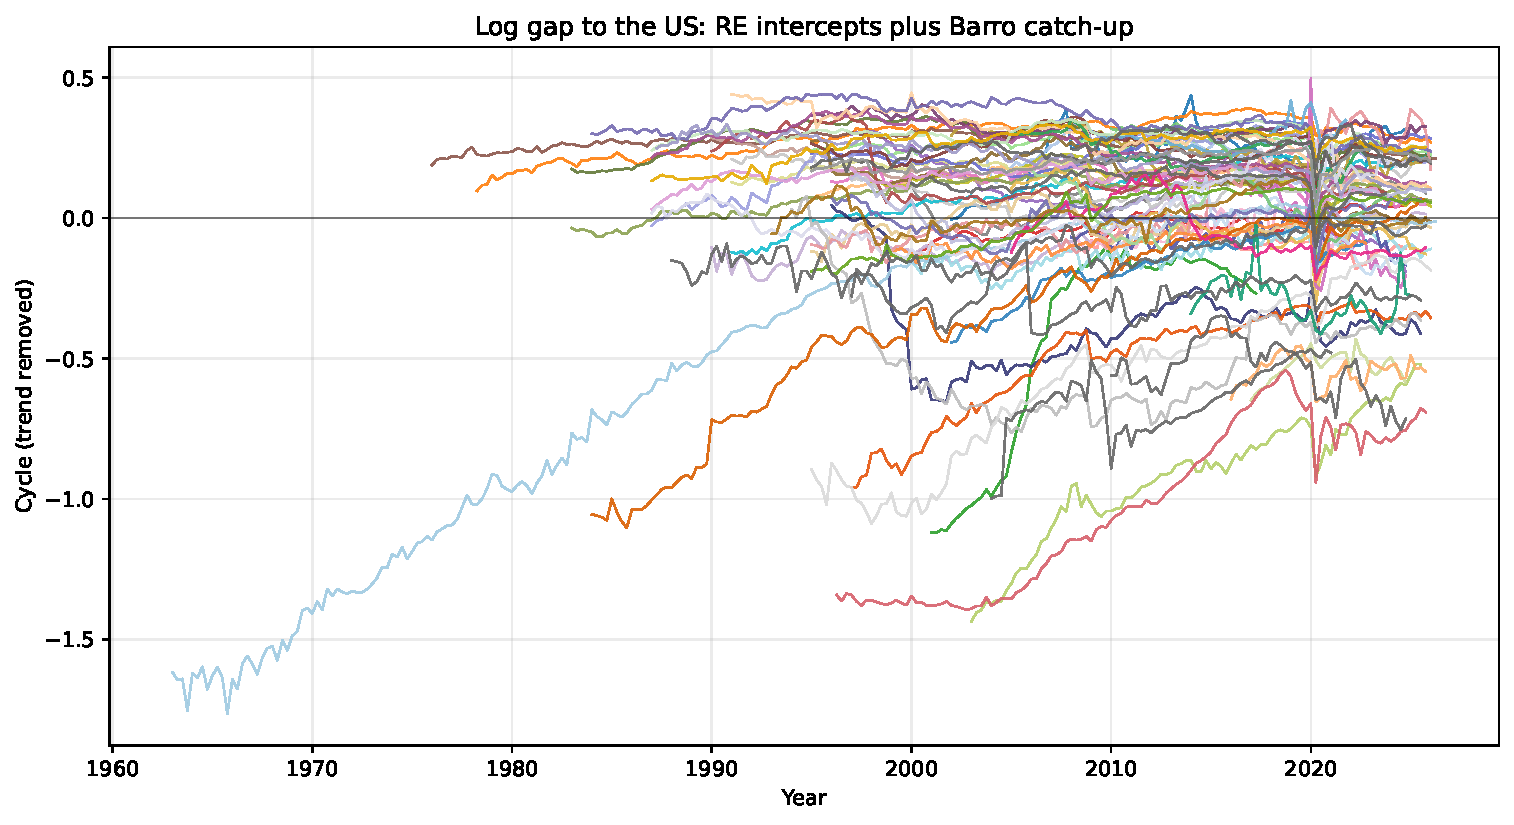
\includegraphics[width=0.75\textwidth]{figs/cycle_gap_barro.pdf}
\caption{Country cycles in the US gap after removing the deterministic path.}
\end{figure}
\end{document}
